%
% 2-transversal.tex
%
% (c) 2023 Prof Dr Andreas Müller
%
\section{Freie Randbedingungen und Transversalität
\label{buch:nebenbedingungen:section:transversl}}
\kopfrechts{Freie Randbedingungen und Transversalität}
Bis jetzt wurden ausschliesslich Anfangspunkt-Endpunkt-Probleme gelöst.
Sie zeichnen sich dadurch aus, dass die Funktion $\eta(x)$, mit der
variiert wurde, in den Endpunkten des Definitionsintervalls
verschwinden.
Dies bedeutet, dass das Verhalten der Funktion in den Endpunkten des
Intervalls kaum einen Einfluss auf die Lösung haben.
Die einzige, durch die Lösungsfunktion zu erfüllende Bedingung ist die
Euler-Lagrange-Gleichung.
Die Anforderung, dass die Endpunkte vorgegeben sind, soll in diesem
Abschnitt aufgeweicht und die Lösung Anfangskurve-Endpunkt-,
Anfangspunkt-Endkurve- und Anfangskurve-Endkurve-Problemen dargestellt
werden.
Dazu ist nötig, zusätzliche Information über das Verhalten der Lösung
am Intervallende aus der allgemeinen Form der Variation zu gewinnen.

Ausserdem mussten bisher studierte Variationsprobleme nur ein 
Integral der Lagrange-Funktion minimieren.
In der Praxis treten jedoch auch Probleme auf, in denen das zu
minimierende Funktional nicht nur ein Integral über den Definitionsbereich
ist, sondern zusätzliche Terme in den Endpunktkoordinaten enthält.
Die Bildung eines Meniskus an einer Flüssigkeitsoberfläche in einer 
Kapillare ist ein solches Problem.
Im Abschnitt~\ref{buch:nebenbedingungen:transversal:subsection:randterme}
wird gezeigt, wie solche Probleme gelöst werden können.

%
% Transversalitätsbedingung
%
\subsection{Transversalitätsbedingung
\label{buch:nebenbedingungen:transversal:subsection:transversalitaetsbedingung}}
In diesem Abschnitt sollen Variationsprobleme gelöst werden, in denen
mindestens ein Endpunkt nicht fest ist sondern auf einer Kurve
varieren kann.

%
% Aufgabenstellung
%
\subsubsection{Aufgabenstellung}
Wir betrachten ein Anfangskurve-Endkurve-Problem mit einer unabhängigen
Variablen in der folgenden Form.

\begin{definition}
\label{buch:nebenbedingungen:transversal:def:zwischenkurven}
Zu gegebenen differenzierbaren Kurven
\begin{align*}
\alpha&\colon I_\alpha\to\mathbb{R}:\alpha \mapsto \gamma_1(\alpha)=(x_1(\alpha),y_1(\alpha)
\intertext{und}
\beta&\colon I_\beta\to\mathbb{R}:\beta\mapsto \gamma_2(\beta)=(x_2(\beta),y_2(\beta)
\end{align*}
heisst eine Funktion $y\colon I\to\mathbb{R}$ Kurve zwischen den beiden
Kurven $\gamma_1$ und $\gamma_2$, wenn es Werte $\alpha_1$ und $\beta_2$ gibt
derart, dass
\begin{align*}
y(x_1(\alpha_1)) &= y_1(\alpha_1)
&&\text{und}&
y(x_1(\beta_1)) &= y_1(\beta_1)
\end{align*}
gilt.
Die Kurve $\gamma_1$ heisst auch die {\em Anfangskurve}, $\gamma_2$
\index{Anfangskurve}%
heisst die {\em Endkurve}.
\index{Endkurve}%
Die beiden Kurven werden auch die {\em Endkurven} des Problems
bezeichnet.
Die {\em Endpunkte} einer Kurve $y(x)$ zwischen den beiden Kurven sind
\index{Endpunkt}%
die Punkte $\gamma_1(\alpha_1)=(x_1(\alpha_1),y_1(\alpha_1))$
und $\gamma_2(\beta_2)=(x_2(\beta_2),y_2(\beta_2))$, in denen die
Kurve $y(x)$ auf die Kurven $\gamma_1$ bzw.~$\gamma_2$ trifft.
\end{definition}

Als besonderer Spezialfall gilt der Fall, in dem $x_1(\alpha)$ oder
$x_2(\beta)$ konstant sind.
In diesem Fall ändert das Definitionsintervall nicht, eine Kurve
zwischen den beiden Endkurven ist immer das Intervall
$I=[x_1(\alpha),x_2(\beta)]$ ganz unabhängig von den Werten von
$\alpha$ und $\beta$.

Eine Kurve zwischen den Kurven $\gamma_1$ und $\gamma_2$ ist eine
mögliche Lösung eines Anfangskurve-Endkurve-Problems mit Anfangskurve
$\gamma_1$ und Endkurve $\gamma_2$.
\index{Anfangskurve-Endkurve-Problem}%
Der Definitionsbereich von $y(x)$ hängt vom Punkt ab, in dem eine Kurve
zwischen den beiden Kurven $\gamma_1$ und $\gamma_2$ auf die beiden
Endkurven trifft.
Da die Endpunkte nicht festgelegt sind, sondern auf den Endkurven
varieren können, muss der Definitionsbereich der Lagrange-Funktion
jedes mögliche $x$-Intervall beinhalten, welches für verschiedene
Werte von $\alpha$ und $\beta$ entstehen kann.
Für den Definitionsbereich $I\times\mathbb{R}\times\mathbb{R}$  der
Lagrange-Funktion $L(x,y,y')$ muss also
\[
[x_1(\alpha),x_2(\beta)]\subset I
\qquad\forall \alpha\in I_\alpha\wedge \beta\in I_\beta
\]
gelten.
Eine Lagrange-Funktion mit dieser Eigenschaft soll für die Zwecke
der folgenden Diskussion ein {\em zulässige} Lagrange-Funktion
genannt werden.

\begin{aufgabe}
\label{buch:nebenbedingungen:transversal:aufgabe:allg}
Gegeben sind zwei Kurven $\gamma_1$ und $\gamma_2$ wie in
Definition~\ref{buch:nebenbedingungen:transversal:def:zwischenkurven}
und eine zulässige Lagrange-Funktion 
\[
F\colon I\times \mathbb{R}\times\mathbb{R}\to\mathbb{R}
: (x,y,y') \mapsto L(x,y,y').
\]
Gesucht ist eine Funktion $y(x)$ und Werte $\alpha$ und $\beta$ derart,
dass $y(x_1(\alpha)) = y_1(\alpha)$ und $y(x_2(\beta))=y_2(\beta)$
und so, dass das Integral
\begin{equation}
I(y)
=
\int_{x_1(\alpha)}^{x_2(\beta)} 
F(x,y(x),y'(x))
\,dx
\label{buch:nebenbedingungen:transversal:eqn:integral}
\end{equation}
unter allen Funktionen extremal ist, 
\end{aufgabe}

%
% Bedingung an die Endpunkte
%
\subsubsection{Bedingung an die Endpunkte}
Die Aufgabenstellung~\ref{buch:nebenbedingungen:transversal:aufgabe:allg}
legt die Endpunkte der Lösungskurve nicht fest.
Wenn wir die Endpunkte bereits kennen würden, dann würde sich die
Aufgabenstellung in ein Anfangs\-punkt-End\-punkt-Problem verwandeln und
es könnte mit der Euler-Lagrange-Differential\-gleichung der Lagrange-Funktion
$L$ gelöst werden.
Zu jedem Paar von Parameterwerten $\alpha$ und $\beta$ ergeben sich
zwei Punkte $\gamma_1(\alpha)$ und $\gamma_2(\beta)$, zwischen denen
eien Lösung zu finden ist.
Es bleibt dann nur noch das Problem zu lösen, $\alpha$ und $\beta$ so
zu bestimmen, dass das
Integral~\eqref{buch:nebenbedingungen:transversal:eqn:integral}
minimal wird.
Diese Vorgehensweise ist aber eher kompliziert, es ist meistens nicht
einfach, den Wert des Integrals direkt durch $\alpha$ und $\beta$
auszudrücken.

Die allgemeine Lösung der Euler-Lagrange-Differentialgleichung enthält
zwei Integrationskonstanten, die so gewählt werden müssen, dass die
Anfangs- oder Randbedingungen erfüllt werden.
Die allgemeine Lösung trifft die Endkurven $\gamma_1$ und $\gamma_2$
in zwei Punkten, die durch die zugehörigen Parameter $\alpha$ und $\beta$
charakterisiert sind.
Es gibt also einen Zusammenhang zwischen den Integrationskonstanten der
allgemeinen Lösung und den Parametern der Randkurve.
Dieser ist nicht unbedingt einfacher, als der Zusammenhang zwischen den
Parametern und dem Wert des Integrals.

Gesucht ist daher eine Methode, die Integrationskonstanten zu bestimmen
erlaubt, ohne dass dazu die Abhängigkeit von den Kurvenparametern bekannt
sein muss.
Die kürzeste Verbindung zwischen einem Punkt und einer Ebene ist die
Gerade durch den Punkt, die auf der Ebene senkrecht steht.
Die Orthogonalität ist also eine geometrische Bedingung über den Endpunkt
der Kurve auf der Ebene, die den Endpunkt vollständig festlegt, ohne dass
dazu die Abhängikgeit der Kurvenlänge vom Endpunkt bekannt sein muss.
Eine Bedingung dieser Art würde einen Zusammenhang zwischen der Richtung
der Kurve $y(x)$ an den Endpunkten und den Tangentialvektoren
\[
\vec{r}_0(\alpha)
=
\frac{d}{d\alpha}\gamma_0(\alpha)
\qquad\text{und}\qquad
\vec{r}_1(\beta)
=
\frac{d}{d\beta}\gamma_1(\beta)
\]
an die Endkurven herstellund.
Mit einer solchen Bedingung könnten $\alpha$ und $\beta$ bestimmt und
damit auch die
Aufgabe~\ref{buch:nebenbedingungen:transversal:aufgabe:allg}
gelöst werden.

Die allgemeine Variationsformel von
Satz~\ref{buch:variation:allgemein:satz:allgemeinvariation1}
liefert die gesuchte Bedingung.
Die Variationsformel~\eqref{buch:variation:allgemein:eqn:allgemeinvariation1}
enthält zusätzlich zum vertrauten Integral zwei Terme, die aber nur von
den Endpunkten abhängt.
Da die extremale Kurve zwischen bekannten Endpunkten den
Euler-Lagrange-Differentialgleichungen genügen muss, verschwindet dieses
Integral und es bleibt
\[
\delta I
=
\vec{f}_1\cdot\vec{r}_1 - \vec{f}_0\cdot\vec{r}_0.
\]
Die Variation hängt jetzt nur noch von den zwei Parametern
$\alpha$ und $\beta$ ab, und zwar hängt der erste Term auf der rechten
Seite nur von $\beta$ ab, der zweite nur von $\alpha$.
Sie entsprechen den Komponenten des Gradienten der Funktion
$I(\alpha,\beta)$, wir müssen daher sicherstellen, dass beide
verschwinden.

So erhalten wir die folgenden sogenannten {\em Transversalitätsbedingungen}
an die Lösung der Aufgabe~\ref{buch:nebenbedingungen:transversal:aufgabe:allg}.
\index{Transversalitätsbedingung}%

\begin{satz}[Transversalität]
\label{buch:nebenbedingungen:transversal:satz:transversal}
\index{Transversalität}%
Eine Lösung $y\colon [x(\alpha),x(\beta)]\to \mathbb{R}$ der 
Aufgabe~\ref{buch:nebenbedingungen:transversal:aufgabe:allg}
löst die Euler-Lagrange-Differentialgleichung und erfüllt ausserdem
die Bedingungen
\begin{equation}
\vec{r}_i\cdot\vec{f}_i=0.
\end{equation}
Der Tangentialvektor $\vec{r}_i$ steht also senkrecht auf dem Vektor,
\begin{equation}
\vec{f}_i
=
\begin{pmatrix}
\displaystyle 
F(x_i, y(x_i),y'(x_i))-y'(x_i)\frac{\partial F}{\partial y'}(x_i,y(x_i),y'(x_i))
\\[3pt]
\displaystyle 
\frac{\partial F}{\partial y'}(x_i,y(x_i),y'(x_i))
\end{pmatrix},
\end{equation}
der allein durch die Werte $x_0 = x_0(\alpha)$ und $x_1=x_1(\beta)$
und die Lösungsfunktion $y(x)$ bestimmt ist.
\end{satz}

%
% Beispiel
%
\subsubsection{Beispiel}
Als Beispiel für die Transversalität lösen wir die Aufgabe, die kürzeste
Verbindung zwischen zwei parallelen Geraden in der Ebene zu finden.
Das zu minimierende Funktional ist 
\[
I(y)
=
\int_{x_0}^{x_1} F(x,y(x),y'(x))\,dx
=
\int_{x_0}^{x_1} \sqrt{1+y'(x)^2}\,dx
\]
mit der Lagrange-Funktion
\[
F(x,y,y')
=
\sqrt{1+y^{\prime 2}}.
\]
Die zugehörige Euler-Lagrange-Differentialgleichung ist 
\[
0
=
\frac{\partial F}{\partial y} - \frac{d}{dx}\frac{\partial F}{\partial y'}
=
0
-
\frac{d}{dx}
\frac{y'}{\sqrt{1+y^{\prime 2}}}
=
-
\frac{y''}{(1+y^{\prime 2})^{\frac32}}.
\]
Nach Satz~\ref{buch:nebenbedingungen:transversal:satz:transversal}
muss sie für die Lösung erfüllt sein, es muss also $y''=0$ gelten.
Lösungen sind also Geraden $y(x)=ax+b$ mit $y'=a$.

Der Richtungsvektor der Randgeraden sei
\[
\vec{r}_0
=
\vec{r}_1
=
\vec{r}
=
\begin{pmatrix}r_x\\r_y\end{pmatrix}.
\]
Um Satz~\ref{buch:nebenbedingungen:transversal:satz:transversal}
anzuwenden, müssen jetzt auch noch die Vektoren $\vec{f}_i$ bestimmt
werden.
Dazu wird die Ableitung
\[
\frac{\partial F}{\partial y'}
=
\frac{y'}{\sqrt{1+y^{\prime 2}}}
=
\frac{a}{\sqrt{1+a^2}}
\]
benötigt.
Für $\vec{f}_i$ ergibt sich damit
\begin{align*}
\vec{f}_i
&=
\begin{pmatrix}
\displaystyle
F(x_i,y(x_i),y'(x_i))
-
y'(x_i)
\frac{\partial F}{\partial y'}(x_i,y(x_i),y'(x_i))
\\[3pt]
\displaystyle
\frac{\partial F}{\partial y'}(x_i,y(x_i),y'(x_i))
\end{pmatrix}
\\
&=
\begin{pmatrix}
\displaystyle
\sqrt{1+a^2} -a\frac{a}{\sqrt{1+a^2}}
\\[3pt]
\displaystyle
\frac{a}{\sqrt{1+a^2}}
\end{pmatrix}
=
\frac{1}{\sqrt{1+a^2}}
\begin{pmatrix}
(1+a^2) -a^2\\
a
\end{pmatrix}
=
\frac{1}{\sqrt{1+a^2}}
\begin{pmatrix}
1\\
a
\end{pmatrix}.
\end{align*}
Die Transversalitätsbedingung $\vec{r}_i\cdot\vec{f}_i=0$ wird damit zu
\[
0
=
\vec{r}_i\cdot\vec{f}_i
=
\begin{pmatrix}
r_x\\r_y
\end{pmatrix}
\cdot
\frac{1}{\sqrt{1+a^2}}
\begin{pmatrix}
1\\
a
\end{pmatrix}
=
\frac{r_x+ar_y}{\sqrt{1+a^2}}
\quad\Rightarrow\quad
a
=
-\frac{r_y}{r_x},
\]
die Steigung von $y(x)$ ist so, dass die Gerade in den Endpunkten senkrecht
auf den Tangentialvektoren $\vec{r}_i$ ist.

%
% Randterme
%
\subsection{Randterme
\label{buch:nebenbedingungen:transversal:subsection:randterme}}
In diesem Abschnitt sollen Variationsproblem gelöst werden, in denen
nicht nur ein Integral minimiert werden soll, sondern ein Funktional,
welches zusätzlich von den Randpunkten abhängig ist.

%
% Aufgabenstellung
%
\subsubsection{Aufgabenstellung}
In einem Anfangspunkt-Endpunkt-Problem muss die Lösung einen Punkt
$\gamma_0(\alpha)$ auf einer mit $\alpha$ parametrisierten Anfangskurve
und $\gamma_1(\beta)$ auf einer mit $\beta$ parametrisierten Endkurve
miteinander verbinden.
Die beiden Parameter $\alpha$ und $\beta$ sind im Rahmen der Problemlösung
ebenfalls zu bestimmen.
Satz~\ref{buch:nebenbedingungen:transversal:satz:transversal}
formuliert eine Bedingung, mit diese Parameter bestimmt werden können.
Ein ähnliches Problem liegt vor, wenn die Intervallenden zwar fest sind,
aber das Funktional
\[
I(y)
=
\int_{x_0}^{x_1}
F(x,y(x),y'(x))
\,dx
+
f_1(y(x_1))
-
f_0(y(x_0))
\]
zusätzlich von Werten von $y(x)$ an den Endpunkten des Intevalls
abhängt.
Die beiden Funktionen $f_0$ und $f_1$ heissen auch die {\em Randterme}
\index{Randterm}%
des Funktionals $I(y)$.

\begin{aufgabe}
\label{buch:nebenbedingungen:transversal:aufgabe:randterme}
Finde eine Funktion $y\colon[x_0,x_1]\to\mathbb{R}$, die das Funktional
\begin{equation}
I(y)
=
\int_{x_0}^{x_1}
F(x,y(x),y'(x))\,dx
+
f_1(y(x_1))
-
f_0(y(x_0))
\label{buch:nebenbedingungen:transversal:eqn:randterme}
\end{equation}
extremal macht.
\end{aufgabe}

%
% Variation für ein Funktional mit Randtermen
%
\subsubsection{Variation für ein Funktional mit Randtermen}
Für die Lösung der
Aufgabe~\ref{buch:nebenbedingungen:transversal:aufgabe:randterme}
berechnen wir wie gewohnt die Variation mit einer Funktion
$\eta:[x_0,x_1]\to\mathbb{R}$, wobei wir aber nicht annehmen dürfen,
dass $\eta$ an den Intervallenden verschwindet.
Die Variation ist
\begin{align*}
\frac{d}{d\varepsilon}I(y+\varepsilon\eta)
\bigg|_{\varepsilon=0}
&=
\int_{x_0}^{x_1}
\frac{\partial F}{\partial y}(x,y(x),y'(x))\eta(x)
+
\frac{\partial F}{\partial y'}(x,y(x),y'(x))\eta'(x)
\,dx
\\
&\qquad
+
f_1'(y(x_1))\eta(x_1)
-
f_0'(y(x_0))\eta(x_0).
\intertext{Durch partielle Integration erhalten wir}
&=
\int_{x_0}^{x_1}
\biggl(
\frac{\partial F}{\partial y}(x,y(x),y'(x))
+
\frac{d}{dx}
\frac{\partial F}{\partial y'}(x,y(x),y'(x))
\biggr)\eta(x)
\,dx
\\
&\qquad
+
\biggl[
\frac{\partial F}{\partial y'}(x,y(x),y'(x))\eta(x)
\biggr]_{x_0}^{x_1}
+
f_1'(y(x_1))\eta(x_1)
-
f_0'(y(x_0))\eta(x_0).
\end{align*}
Für Variationen $\eta$, die in den Endpunkten des Intervalls verschwinden,
bleibt nur der Integralterm.
Da die Variation für alle solchen Variationen verschwinden muss,
gilt also für die Lösung $y(x)$ weiterhin die
Euler-Lagrange-Differentialgleichung.

Wir betrachten jetzt Variationen $\eta$, die am Intervallende nicht
verschwinden.
Die Funktionen 
\[
\eta_0(x)
=
\frac{
g_{x_0-\varepsilon,x_0+\varepsilon}(x)
}{
g_{x_0-\varepsilon,x_0+\varepsilon}(x_0)
}
\qquad\text{und}\qquad
\eta_1(x)
=
\frac{
g_{x_1-\varepsilon,x_1+\varepsilon}(x)
}{
g_{x_1-\varepsilon,x_1+\varepsilon}(x_0)
}
\]
für $x$ im Intervall $[x_0,x_1]$ sind beliebig oft stetig differenzierbar
und nehmen die Werte
\begin{align*}
\eta_0(x_0) &= 1 & \eta_0(x_1) &= 1
\\
\eta_1(x_0) &= 0 & \eta_1(x_1) &= 1
\end{align*}
und haben die Träger
\begin{align*}
\operatorname{supp}\eta_0 &= [x_0,x_0+\varepsilon]
&&\text{und}&
\operatorname{supp}\eta_1 &= [x_1-\varepsilon,x_1],
\end{align*}
sie sind also zulässige Variationen.
Da für die Funktion $y(x)$  Euler-Lagrange-Differential\-gleichung
gilt, trägt das Integral nichts zur Variation bei, es bleibt dann nur
\begin{align*}
\delta I(y)
&=
-\frac{\partial F}{\partial y'}\bigl(x_0,y(x_0),y'(x_0)\bigr) - f_0'(y(x_0))
&&\text{für $\eta_0$}
\intertext{und}
\delta I(y)
&=
\phantom{-}\frac{\partial F}{\partial y'}\bigl(x_1,y(x_1),y'(x_1)\bigr) + f_1'(y(x_1))
&&\text{für $\eta_1$.}
\end{align*}
Da $\delta I$ auch für diese Funktionen $\eta_i$ verschwinden müssen,
ergibt sich der folgende Satz.

\begin{satz}
\label{buch:nebenbedingungen:transversal:satz:randterme}
Das Funktional
\eqref{buch:nebenbedingungen:transversal:eqn:randterme}
wird extremal für Funktionen $y(x)$, die die
Euler-La\-gran\-ge-Differentialgleichung für die Lagrange-Funktion $F$ erfüllen
und ausserdem die Bedingungen
\begin{align}
\frac{\partial F}{\partial y'}\bigl(x_0,y(x_0),y'(x_0)) &= -f_0'(y(x_0)\bigr)
&&\text{und}&
\frac{\partial F}{\partial y'}\bigl(x_1,y(x_1),y'(x_1)) &= -f_1'(y(x_1)\bigr)
\label{buch:nebenbedingungen:transversal:eqn:randtermbed}
\end{align}
erfüllen.
\end{satz}

Die allgemeine Lösung der Euler-Lagrange-Differentialgleichung
enthält zwei Integrationskonstanten, die normalerweise durch
Randbedingungen festgelegt würden.
Setzt man die allgemeine Lösung in die Gleichungen
\eqref{buch:nebenbedingungen:transversal:eqn:randtermbed}
ein, ergeben sich zwei Gleichungen für die Integrationskonstanten.

%
% Beispiel: Meniskus
%
\subsubsection{Beispiel: Meniskus}
\index{Meniskus}%
Als Beispiel für eine Aufgabe mit Randtermen betrachten wir das
Problem, die Form und Höhe des Meniskus, den eine Flüssigkeit zwischen
zwei vertikalen, parallelen ebenen Flächen unter der Wirkung der
Schwerkraft und der Oberflächenspannung bildet.
\index{Schwerkraft}%
\index{Oberflächenspannung}%

Die potentielle Energie der Flüssigkeit mit Dichte $\varrho$, die 
\index{potentielle Energie}%
durch die Funktion $y(x)$ im Intervall $[-l,l]$ berandet ist, ist
\[
\int_{-l}^l
\frac12
\varrho
g
y(x)^2
\,dx.
\]
Dazu kommt die Energie der Oberflächenspannung
\[
\int_{-l}^l \sqrt{1+y^{\prime 2}}\,dx
\]
der Flüssigkeitsoberfläche entlang der Kurve $y(x)$, die 
proportional zur Kurvenoberfläche ist.
Dazu kommt die Oberflächenenergie, die durch die Benetzung der
beiden berandenden Ebenen durch die Flüssigkeit entsteht, die
proportional zur benetzten Fläche ist. 
Sie trägt einen Term
\[
\sigma y(-l) + \sigma y(l)
=
\sigma(y(-l)+y(l))
\]
bei.
Das zu minimierende Funktion ist daher
\[
I(y)
=
\int_{-l}^l
\frac12\varrho g y(x)^2
+
\sqrt{1+y'(x)^2}
\,dx
+
\sigma(y(-l)+y(l))
\]
mit der Lagrange-Funktion
\[
L(x,y,y')
=
\frac12\varrho g y^2
+
\sqrt{1+y^{\prime 2}}
\]
und den Randtermen
\[
f_0(y) = -\sigma y
\qquad\text{und}\qquad
f_1(y) = \sigma y.
\]

%
% meniskus.tex
%
% (c) 2024 Prof Dr Andreas Müller
%
\begin{figure}
\centering
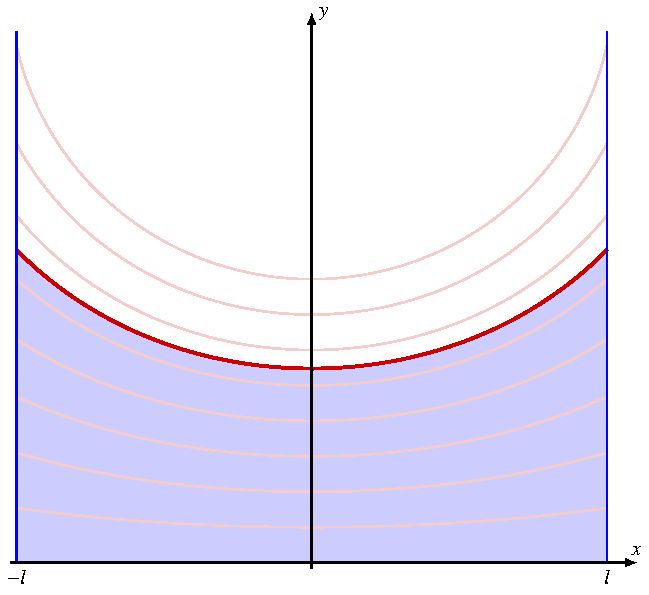
\includegraphics{chapters/050-nebenbedingungen/images/meniskus.pdf}
\caption{Meniskus zwischen zwei parallelen, vertikalen Ebenen
im Abstand $2l$.
Je grössser $\sigma$ ist, desto höher steigt die Flüssigkeitsoberfläche
und desto steiler trifft die Oberfläche auf die Wand.
\label{buch:nebenbedingungen:transversal:fig:meniskus}}
\end{figure}


Die Euler-Lagrange-Differentialgleichung für die Lagrange-Funktion entsteht
aus den partiellen Ableitungen
\[
\frac{\partial L}{\partial y}
=
\varrho g y
\qquad\text{und}\qquad
\frac{\partial L}{\partial y'}
=
\frac{y'}{\sqrt{1+y^{\prime 2}}}
\]
und lautet
\begin{align*}
0
&=
\varrho g y(x)
-
\frac{d}{dx}
\frac{y'(x)}{\sqrt{1+y'(x)^2}}
\\
&=
\varrho g y(x)
-
\frac{ y''(x) }{(1+y'(x)^2)^{\frac32}}.
\end{align*}
Die Randbedingungen sind
\begin{align*}
\frac{y'(-l)}{\sqrt{1+y'(-l)^2}}
=
\frac{\partial L}{\partial y'}(-l,y(-l),y'(-l)) &= f_0'(y(-l)) = -\sigma
\\
\frac{y'(l)}{\sqrt{1+y'(l)^2}}
=
\frac{\partial L}{\partial y'}(l,y(l),y'(l)) &= f_1'(y(l)) = \sigma,
\end{align*}
dies sind Gleichungen, mit denen die Steigung $y'(\pm l)$ am Rand ermittelt
werden kann.
Schreibt man $\pm \varphi$ für den Winkel, mit dem der Meniskus auf
den Rand trifft, dann ist
\[
\tan\varphi
=
y'(l)
\qquad
\Rightarrow
\qquad
\sin\varphi
=
\frac{y'(l)}{\sqrt{1+y'(l)}}
=
\sigma.
\]
Der Winkel $\varphi$ hängt also nur von der Konstanten $\sigma$ ist.

%
% Meniskus in einer Kapillare
%
\subsubsection{Meniskus in einer Kapillare}
Für das Problem des Meniskus, der sich bildet, wenn eine Flüssigkeit
in einer Kapillare vom Radius $a$ hochsteigt, werden Zylinderkoordinaten
\index{Kapillare}
$(\varphi,r,z)$ verwendet.
Für eine rotationssymmetrische Lösung muss nur die Funktion $z(r)$ 
bestimmt werden, mit der sich die Energie als
\[
I(z)
=
2\pi
\int_0^a
\frac12
\varrho g
z(r)^2
r
\,dr
+
2\pi
\int_0^a
\sqrt{1+z'(r)^2}
r\,dr
+
2\pi a
\sigma z(a)
\]
mit der Lagrange-Funktion
\[
\frac{1}{2\pi}
L(r, z, z')
=
\frac12
\varrho g
r
z^2 
+
r
\sqrt{1+z^{\prime 2}}
\]
und den Randterm
\[
f_1(z) = 2\pi a \sigma z.
\]
Da nur ein Randterm vorliegt, ist noch eine weitere Bedingung notwendig,
um die Lösung zu bestimmen.
Sie ergibt sich daraus, dass die Funktion $z(r)$ auf der Achse der Kapillare
bei $r=0$ ein glatte Fläche beschreiben soll, was nur möglich ist, wenn dort
$z'(0)=0$ gilt.

Für die Euler-Lagrange-Differentialgleichung für die Lagrange-Funktion $L$
müssen erst die partiellen Ableitungen
\[
\frac{\partial L}{\partial z}
=
\varrho g r z
\qquad\text{und}\qquad
\frac{\partial L}{\partial z'}
=
\frac{rz'}{\sqrt{1+z^{\prime 2}}}
\]
ermittelt werden.
Die Differentialgleichung ergibt sich daraus als
\begin{align*}
0
&=
\varrho grz
-
\frac{d}{dr}
\frac{rz'(r)}{\sqrt{1+z'(r)^2}}
\\
&=
\varrho grz
-
\frac{
\displaystyle
(z'(r)+rz''(r))\sqrt{1+z'(r)^2}
-
rz'(r)\frac{z'(r)}{\sqrt{1+z'(r)^2}}z''(r)
}{
1+z'(r)^2
}
\\
&=
\varrho grz
-
\frac{
z'(r)(1+z'(r)^2)
+
rz''(r)(1+z'(r)^2)
-
rz'(r)^2z''(r)
}{
(1+z'(r)^2)^{\frac32}
}
\\
&=
\varrho grz
-
\frac{
z'(r)(1+z'(r)^2)
+
rz''(r)
}{
(1+z'(r)^2)^{\frac32}
},
\end{align*}
die allerdings nicht in geschlossener Form gelöst werden kann, selbst
mit der Randbedingung $z'(0)=0$.

Die Bedingung für die Steigung am Rand ergibt sich aus dem Randterm
\begin{align*}
\frac{\partial L}{\partial z'}(a, z(a), z'(a))
&=
-
f_1'(z(a))
\\
2\pi a
\frac{z'(a)}{\sqrt{1+z'(a)^2}}
&=
2\pi a \sigma
\qquad\Rightarrow\qquad
\sin\alpha = \sigma.
\end{align*}
Es ergibt sich also die gleiche Formel für den Berührungswinkel wie
\index{Berührungswinkel}%
im ebenen Fall.




